\documentclass{article}

\usepackage{geometry}
\usepackage{url} 
\usepackage{listings}
\usepackage{xcolor}
\usepackage{nth}
\usepackage{graphicx}

\title{ RSA digital signature -- documentation}
\author{Maciej Marcinkiewicz, Katarzyna Bielecka}
\date{\nth{20} January 2022}

\newgeometry{lmargin=3.2cm, rmargin=3.2cm, bmargin=2.5cm}

\lstset{
    tabsize=4, % tab space width
    showstringspaces=false, % don't mark spaces in strings
    basicstyle=\ttfamily,
    keywordstyle=\color{blue}\ttfamily,
    stringstyle=\color{red}\ttfamily,
    commentstyle=\color{green}\ttfamily
}

\begin{document}

\maketitle

\section{Description of the used algorithm}
% short theory
RSA (Rivest-Shamir-Adleman) is a public key cryptosystem, which was invented in 1977. It is not the newest one but it is still commonly used for securing data transmisson.
It can be used both for encryption as well as for digital signatures. In general, it makes use of the integer factorization problem, which in number theory is the decomposition of a composite number into a product of smaller integers. In case of these integers being prime it is then called prime factorization.  

\section{Functional description of the application}
% input data formats, outputs etc.
The RSA cryptosystem application provides the following functionalities:
public and private key generation, digital signature generation and signature verification.
Below, algorithms needed for each of those functionalities are described.

\subsection{Keys generation}
\begin{enumerate}
    \item Generate two random, large prime numbers \textbf{p} and \textbf{q}
    \item Compute $ n = p*q $  and $ \phi = (p - 1)*(q - 1) $
    \item Find \textbf{e}, such that  $ 1 < e < \phi$ and $\gcd(e,\phi) = 1 $
    \item Using the extended Euclidean algorithm produce a unique \textbf{d}, such that $ 1 < d < \phi $  and $ e*d \equiv  1 $(mod $\phi$)  
    \item (n,e) is the resulting public key and d is the private key
\end{enumerate}

\subsection{Signature generation}
\begin{enumerate}
    \item Compute $  h = sha512(m) $ where \textbf{h} is the hash of the message \textbf{m}  
    \item Compute $ s = h^d $ (mod $n$)
    \item \textbf{s} is the generated signature
\end{enumerate}

\subsection{Signature verification}
\begin{enumerate}
    \item Compute $\tilde{h} = s^e $ (mod $n$)
    \item Compute $  h = $sha512 $(m) $ where \textbf{h} is the hash of the message \textbf{m}
    \item If $\tilde{h}$ is equal to h then the signature is valid

\end{enumerate}

\newpage

\section{Description of designed code structure}
\subsection{Miller-Rabin primality test}
\subsubsection{Code}

\small
\begin{lstlisting}[language=Python]
    def is_prime(n: int, k: int) -> bool:
    """
    The function implements the Miller-Rabin primality test.

    Input:
    n - the number to be tested
    k - number of tests to be performed

    Output: a boolean value
    """

    # trivial cases: 0-2 and even numbers
    if n == 2:
        return True
    elif n <= 1 or n % 2 == 0:
        return False

    # writing n as 2^r * d + 1 with d odd
    r = 0
    d = n - 1
    while d % 2 == 0:
        d //= 2
        r += 1

    # perform k number of tests
    for _ in range(k):
        a = randrange(2, n - 2)
        x = pow(a, d, n)

        if x == 1 or x == n - 1:
            continue

        for _ in range(r - 1):
            x = pow(x, 2, n)
            if x == n - 1:
                break
        else:
            return False

    return True
\end{lstlisting}
\normalsize

\subsubsection{Description}
The first key component of the program (and of the most of cryptographic software) is the primality
checker. As RSA requires two distinct large prime numbers, there is a need for an efficient algorithm.
Simply iterating through every number up half of tested numbers and checking remainder of
division operation would not be very effective.

The Miller-Rabin primality test is a perfect solution to this problem. It is a probabilistic algorithm, so
for certain numbers it could give wrong results. To prevent this, the algorithm is executed in several rounds.
Each of them increases certainty of the test's result.

In the beginning, the function rejects trivial cases of numbers -- the first three natural numbers
and even numbers. It is obvious that they are not prime thus in a lot of cases the function can finish its
execution earlier. Tested numbers are randomly generated, it means that in c.a. half of given cases
function will end faster.

Next, the tested number has to be transformed into $2^r \cdot d + 1$ form. After that step, the
test is performed k-times.

\subsection{Large prime number generation}
\subsubsection{Code}

\small

\begin{lstlisting}[language=Python]
    def generate_prime_number(prime_size:int) -> int:
    """
    Generates large prime numbers.

    Input: prime_size - size of prime number expressed in number of bits

    Output: p - a large prime number
    """

    p = 0

    # choose randomly a large number until prime is obtained
    while not is_prime(p, 180):
        p = getrandbits(prime_size)

    return p
\end{lstlisting}

\normalsize

\subsubsection{Description}
The function is mostly based on a primality test. It takes a randomly generated number and
passes it to the Miller-Rabin test function. The random number generation is done by a function from
the standard Python module -- random. Size of those numbers is given in bits to
easily control the size of generated keys, which is also in bits. If the test is passed, value true is returned.
If it is not, the process is repeated until a prime number is obtained.

\subsection{Extended Euclidean algorithm}
\subsubsection{Code}

\small

\begin{lstlisting}[language=Python]
    def extended_euclidean(a: int, b: int) -> tuple[int, int, int]:
    """
    Computes greatest common divisor and the coefficients of `Bézout''s identity.

    Input: a, b - non-negative integers satisfying a >= b

    Output: gcd  - greatest common divisor
            x, y - the coefficients of Bézout's identity
    """

    if b == 0:
        return (a, 1, 0)

    x1, x2, y1, y2 = 0, 1, 1, 0
    while b > 0:
        q, r = divmod(a, b)
        x = x2 - q * x1
        y = y2 - q * y1

        a, b, x2, x1, y2, y1 = b, r, x1, x, y1, y

    gcd, x, y = a, x2, y2
    return (gcd, x, y)
\end{lstlisting}

\normalsize

\subsubsection{Description}
The second algorithm that is needed before the process of RSA keys generation is the extended Euclidean algorithm. 
What makes this version of algorithm special is that it not only computes the greatest common divisor of two numbers, but 
it also yields two coefficients of Bézout's identity $ax + by = gcd(a, b)$. One of these coefficients is the modular multiplicative inverse and 
it makes the extended Euclidean algorithm one of the easiest methods of obtaining this inverse.

\subsection{RSA keys generation}
\subsubsection{Code}

\small

\begin{lstlisting}[language=Python]
    def generate_keys(key_size:int = 2048, return_primes: bool = False)
         -> Union[tuple[int, int, int], tuple[int, int, int, int, int]]:
    """
    Generates RSA public and private keys.

    Input: key_size - size of the key expressed in number of bits (2048 bits by default)
           return_prime - if set, function returns additionaly tuple of prime numbers 
           p and q used in key generation

    Output: (n, e) - public key
                 d - private key
            (p, q) - primes used in generation (optional)
    """

    # generate two large random primes
    p = generate_prime_number(key_size // 2)
    q = generate_prime_number(key_size // 2)

    n = p * q
    fi = (p - 1) * (q - 1)

    # find such e, that e and fi are coprimes
    e = 0
    while gcd(e, fi) != 1:
        e = randrange(1 + 1, fi - 1)

    # find modular multiplicative inverse
    _, x, _ = extended_euclidean(e, fi)
    d = x + fi

    # return public and private keys (optionally primes p and q)
    if return_primes:
        return ((n, e), d, (p, q))
    else:
        return ((n, e), d)
\end{lstlisting}

\normalsize

\subsubsection{Description}
This function generates public and private keys and optionally returns a tuple of prime
numbers that have been used for generation process.

It starts with generating those two primes. Size of the keys is specified thus primes have
to be half of the key's size because they are multiplied one by another in the next step.

After n and $\phi$ are calculated the process of finding e starts. According to theory,
e just has to be coprime with $\phi$. However in real life cases Fermat primes are commonly used. 
Early implementations of RSA were vulnerable to small e exponents and one of the
most common choice for that exponent is 65537 -- the largest known Fermat prime.

The last step is to find modular multiplicative inverse of e and $\phi$ which is finally
a d private exponent. Note that $\phi$ has to be added to the Bézout coefficient in order to get a
proper inverse. Non-negative number is preferred and both x and x + $\phi$ have the same remainder
after division operation, so it is allowed to apply such addition.

\subsection{Signature generation}
\subsubsection{Code}

\small

\begin{lstlisting}[language=Python]
    def generate_signature(m, n: int, e: int, d: int) -> int:
    """
    The function generates an RSA digital signature.

    Input:
    m - message
    n, e - public key of sender
    d - private key of sender

    Output:
    a digital signature s

    """
    # compute hash of message
    h = int(sha512(m.encode("utf-8")).hexdigest(), 16) % 10 ** 8

    # compute signature and return it
    s = pow(h, d, n)
    return s
\end{lstlisting}

\normalsize

\subsubsection{Description}
In order to generate the signature for a given message, the unction just has to compute 
the remainder. Before that, a hash of the message has to be generated (SHA-512 in this case).
The Hash, in the form of an integer is raised to a power of private exponent d. The result is then
divided by n and remainder of this operation is the signature.

This is a very theoretical implementation of the signing. In real-world applications the signatures are padded
to make them less vulnerable to existential forgery attacks. A Commonly used format is PKCS \#1 (part
of standards defined in Public-Key Cryptography Standards). It takes the hash of the message and an
identifier of the hash function, converts to the ASN.1 form and codes them with BER rules. Then
it is formatted in a different way and the octets of that data are converted into one integer.
As this process is not the purpose of the project, that way data formatting will not be described
in this document.

\subsection{Signature verification}
\subsubsection{Code}

\small

\begin{lstlisting}[language=Python]
    def verify(m, n: int, e: int, s: int) -> bool:
    """
    The function generates verifies the received signature using public key.

    Input:
    (n,e) - public key of sender
    s - digital signature

    Output:
    a boolean value

    """
    # decrypt the message
    h_ = pow(s, e, n)

    # calculate message hash
    h = int(sha512(m.encode("utf-8")).hexdigest(), 16) % 10 ** 8

    # compare and return
    return h_ == h    
\end{lstlisting}

\normalsize

\subsubsection{Description}
Process of verification is similar to the signature generation. Verification is passed when
decrypted message's hash is the same as newly generated. In a real-life example it would be also
implemented for instance in PKCS \#1 way.

\section{Tests}
\subsection{Introduction}
All tests have been implemented with use of Python's standard module unittest.
However to run most of the tests a \nth{3}-party PyCryptodome module is required.
It is used as a trusted source for validation.

What also has to be noted is that signature generation and verification functions were not tested
with help of external sources due to the padding format described in the previous section.
Implementation of PKCS \#1 is a whole other task and it out of scope of this project.
If the signing and verification were implemented in such way, they could be verified with utilites
such as ssh-keygen, openssl or earlier mentioned PyCryptodome module.

All tests have been passed and it is documented by the following image.

\newpage

\begin{figure}[h!] %possible: b, t, h, p and override (!)
    \centering
        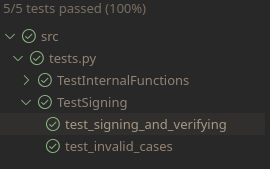
\includegraphics[width=0.5\linewidth]{passed_tests.png}
\end{figure}


\subsection{Test cases}
\subsubsection{Miller-Rabin test}
Prime checker function is tested by generating keys, taking p and q used for their generation
and passing them to PyCryptodome's prime testing function.

\small

\begin{lstlisting}[language=Python]
    def test_primes(self):
        """
        Check if numbers used in keys generation are actually prime.
        """

        # generate primes for testing
        (_, _), _, (p, q) = rsa.generate_keys(return_primes=True)

        # test with PyCryptodome's implementation of Miller-Rabin test
        self.assertTrue(isPrime(p))
        self.assertTrue(isPrime(q))
\end{lstlisting}

\normalsize

\subsubsection{Public exponent}
The correctness of public exponent is assessed by checking if it is a coprime with $\phi$.
For testing purpose \texttt{gcd(a, b)} function from Python's math module has been used.

\small

\begin{lstlisting}[language=Python]
    def test_public_exponent(self):
        """
        Check if public exponent e and phi are coprime numbers.
        """

        # generate public expontent for testing and calculate phi
        (_, e), _, (p, q) = rsa.generate_keys(return_primes=True)
        phi = (p - 1) * (q - 1)

        # test with gcd() function from standard math module
        self.assertTrue(gcd(e, phi))
\end{lstlisting}

\normalsize

\subsubsection{Extended Euclidean algorithm}
In order to check whether the algorithm is implemented correctly, the calculated Bézout coefficients
are plugged into $ax + by$ and compared with the outputs of earlier mentioned \texttt{gcd(a, b)} function.

\newpage

\small

\begin{lstlisting}[language=Python]
    def test_extended_euclidean(self):
        """
        Test whether coefficients of Bézouts identity are valid
        and equation ax + by = gcd(a, b) is fulfilled.
        """

        # generate two random integers to check
        a = randint(10, 1000)
        b = randint(10, 1000)

        # calculate Bézouts coefficients
        _, x, y = rsa.extended_euclidean(a, b)

        # calculate ax + by
        equation_result = a * x + b * y

        # test with gcd() function from standard math module
        self.assertEqual(equation_result, gcd(a, b))
\end{lstlisting}

\normalsize

\subsection{Signature and verification}
Four signatures are generated -- each with different key size. The
signatures are then verified by \texttt{verify(m, n: int, e: int, s: int)} function.

\small

\begin{lstlisting}[language=Python]
    def test_signing_and_verifying(self):
        """
        Test if generated signature for a given message can be
        verified correctly for different sizes of key.
        """

        # message for all tests
        message = ("Lorem ipsum dolor sit amet, consectetur adipiscing elit, ",
                    "sed do eiusmod tempor incididunt ut labore et dolore magna aliqua.")

        # 512-bit key
        (n_512, e_512), d_512 = rsa.generate_keys(512)
        s_512 = rsa.generate_signature(message, n_512, e_512, d_512)

        # 1024-bit key
        (n_1024, e_1024), d_1024 = rsa.generate_keys(1024)
        s_1024 = rsa.generate_signature(message, n_1024, e_1024, d_1024)

        # 2048-bit key
        (n_2048, e_2048), d_2048 = rsa.generate_keys()
        s_2048 = rsa.generate_signature(message, n_2048, e_2048, d_2048)

        # 4096-bit key
        (n_4096, e_4096), d_4096 = rsa.generate_keys(4096)
        s_4096 = rsa.generate_signature(message, n_4096, e_4096, d_4096)

        self.assertTrue(rsa.verify(message, n_512, e_512, s_512))
        self.assertTrue(rsa.verify(message, n_1024, e_1024, s_1024))
        self.assertTrue(rsa.verify(message, n_2048, e_2048, s_2048))
        self.assertTrue(rsa.verify(message, n_4096, e_4096, s_4096))
\end{lstlisting}

\normalsize

\subsubsection{Invalid cases}
Additonally, two cases of wrong usage have been tested. In the first one, the signature is verified with
an incorrect message -- not the one that it has been generated for. In the second case, the given message is correct,
however public key is not -- it is a newly generated one.

\small

\begin{lstlisting}[language=Python]
    def test_invalid_cases(self):
        """
        Test cases when signature verification is not passed.
        """

        # generate signature for a message
        message = "Sample message"
        (n, e), d = rsa.generate_keys()
        s = rsa.generate_signature(message, n, e, d)

        # verify signature for another message
        message2 = "Another message"
        self.assertFalse(rsa.verify(message2, n, e, s))

        # verify the same signature for another public key
        (n, e), d = rsa.generate_keys()
        self.assertFalse(rsa.verify(message, n, e, s))
\end{lstlisting}

\normalsize

\section{Bibliography}
\begin{enumerate}
    \item Menezes, Alfred; van Oorschot, Paul C.; Vanstone, Scott A. (October 1996). Handbook of Applied Cryptography, Chapter 8
    \item \url{https://en.wikipedia.org/wiki/RSA_(cryptosystem)}
    \item \url{https://en.wikipedia.org/wiki/Extended_Euclidean_algorithm}
\end{enumerate}

\end{document}
